% Options for packages loaded elsewhere
\PassOptionsToPackage{unicode}{hyperref}
\PassOptionsToPackage{hyphens}{url}
%
\documentclass[
  landscape]{article}
\usepackage{amsmath,amssymb}
\usepackage{lmodern}
\usepackage{iftex}
\ifPDFTeX
  \usepackage[T1]{fontenc}
  \usepackage[utf8]{inputenc}
  \usepackage{textcomp} % provide euro and other symbols
\else % if luatex or xetex
  \usepackage{unicode-math}
  \defaultfontfeatures{Scale=MatchLowercase}
  \defaultfontfeatures[\rmfamily]{Ligatures=TeX,Scale=1}
\fi
% Use upquote if available, for straight quotes in verbatim environments
\IfFileExists{upquote.sty}{\usepackage{upquote}}{}
\IfFileExists{microtype.sty}{% use microtype if available
  \usepackage[]{microtype}
  \UseMicrotypeSet[protrusion]{basicmath} % disable protrusion for tt fonts
}{}
\makeatletter
\@ifundefined{KOMAClassName}{% if non-KOMA class
  \IfFileExists{parskip.sty}{%
    \usepackage{parskip}
  }{% else
    \setlength{\parindent}{0pt}
    \setlength{\parskip}{6pt plus 2pt minus 1pt}}
}{% if KOMA class
  \KOMAoptions{parskip=half}}
\makeatother
\usepackage{xcolor}
\usepackage[margin=1in]{geometry}
\usepackage{longtable,booktabs,array}
\usepackage{calc} % for calculating minipage widths
% Correct order of tables after \paragraph or \subparagraph
\usepackage{etoolbox}
\makeatletter
\patchcmd\longtable{\par}{\if@noskipsec\mbox{}\fi\par}{}{}
\makeatother
% Allow footnotes in longtable head/foot
\IfFileExists{footnotehyper.sty}{\usepackage{footnotehyper}}{\usepackage{footnote}}
\makesavenoteenv{longtable}
\usepackage{graphicx}
\makeatletter
\def\maxwidth{\ifdim\Gin@nat@width>\linewidth\linewidth\else\Gin@nat@width\fi}
\def\maxheight{\ifdim\Gin@nat@height>\textheight\textheight\else\Gin@nat@height\fi}
\makeatother
% Scale images if necessary, so that they will not overflow the page
% margins by default, and it is still possible to overwrite the defaults
% using explicit options in \includegraphics[width, height, ...]{}
\setkeys{Gin}{width=\maxwidth,height=\maxheight,keepaspectratio}
% Set default figure placement to htbp
\makeatletter
\def\fps@figure{htbp}
\makeatother
\setlength{\emergencystretch}{3em} % prevent overfull lines
\providecommand{\tightlist}{%
  \setlength{\itemsep}{0pt}\setlength{\parskip}{0pt}}
\setcounter{secnumdepth}{-\maxdimen} % remove section numbering
\ifLuaTeX
  \usepackage{selnolig}  % disable illegal ligatures
\fi
\IfFileExists{bookmark.sty}{\usepackage{bookmark}}{\usepackage{hyperref}}
\IfFileExists{xurl.sty}{\usepackage{xurl}}{} % add URL line breaks if available
\urlstyle{same} % disable monospaced font for URLs
\hypersetup{
  pdftitle={Relatório - Avaliação Diagnóstica},
  hidelinks,
  pdfcreator={LaTeX via pandoc}}

\title{Relatório - Avaliação Diagnóstica}
\author{}
\date{\vspace{-2.5em}}

\begin{document}
\maketitle

\hypertarget{resultados.}{%
\section{Resultados.}\label{resultados.}}

\begin{longtable}[]{@{}
  >{\centering\arraybackslash}p{(\columnwidth - 28\tabcolsep) * \real{0.1028}}
  >{\centering\arraybackslash}p{(\columnwidth - 28\tabcolsep) * \real{0.0841}}
  >{\centering\arraybackslash}p{(\columnwidth - 28\tabcolsep) * \real{0.0561}}
  >{\centering\arraybackslash}p{(\columnwidth - 28\tabcolsep) * \real{0.0561}}
  >{\centering\arraybackslash}p{(\columnwidth - 28\tabcolsep) * \real{0.0561}}
  >{\centering\arraybackslash}p{(\columnwidth - 28\tabcolsep) * \real{0.0561}}
  >{\centering\arraybackslash}p{(\columnwidth - 28\tabcolsep) * \real{0.0561}}
  >{\centering\arraybackslash}p{(\columnwidth - 28\tabcolsep) * \real{0.0467}}
  >{\centering\arraybackslash}p{(\columnwidth - 28\tabcolsep) * \real{0.0561}}
  >{\centering\arraybackslash}p{(\columnwidth - 28\tabcolsep) * \real{0.0561}}
  >{\centering\arraybackslash}p{(\columnwidth - 28\tabcolsep) * \real{0.0561}}
  >{\centering\arraybackslash}p{(\columnwidth - 28\tabcolsep) * \real{0.0561}}
  >{\centering\arraybackslash}p{(\columnwidth - 28\tabcolsep) * \real{0.0561}}
  >{\centering\arraybackslash}p{(\columnwidth - 28\tabcolsep) * \real{0.0561}}
  >{\centering\arraybackslash}p{(\columnwidth - 28\tabcolsep) * \real{0.1495}}@{}}
\caption{Aproveitamento das notas entre {[}0,1{]}.}\tabularnewline
\toprule()
\begin{minipage}[b]{\linewidth}\centering
matricula
\end{minipage} & \begin{minipage}[b]{\linewidth}\centering
tipo
\end{minipage} & \begin{minipage}[b]{\linewidth}\centering
1
\end{minipage} & \begin{minipage}[b]{\linewidth}\centering
2
\end{minipage} & \begin{minipage}[b]{\linewidth}\centering
3
\end{minipage} & \begin{minipage}[b]{\linewidth}\centering
4
\end{minipage} & \begin{minipage}[b]{\linewidth}\centering
5
\end{minipage} & \begin{minipage}[b]{\linewidth}\centering
6
\end{minipage} & \begin{minipage}[b]{\linewidth}\centering
7
\end{minipage} & \begin{minipage}[b]{\linewidth}\centering
8
\end{minipage} & \begin{minipage}[b]{\linewidth}\centering
9
\end{minipage} & \begin{minipage}[b]{\linewidth}\centering
10
\end{minipage} & \begin{minipage}[b]{\linewidth}\centering
11
\end{minipage} & \begin{minipage}[b]{\linewidth}\centering
12
\end{minipage} & \begin{minipage}[b]{\linewidth}\centering
aproveitamento
\end{minipage} \\
\midrule()
\endfirsthead
\toprule()
\begin{minipage}[b]{\linewidth}\centering
matricula
\end{minipage} & \begin{minipage}[b]{\linewidth}\centering
tipo
\end{minipage} & \begin{minipage}[b]{\linewidth}\centering
1
\end{minipage} & \begin{minipage}[b]{\linewidth}\centering
2
\end{minipage} & \begin{minipage}[b]{\linewidth}\centering
3
\end{minipage} & \begin{minipage}[b]{\linewidth}\centering
4
\end{minipage} & \begin{minipage}[b]{\linewidth}\centering
5
\end{minipage} & \begin{minipage}[b]{\linewidth}\centering
6
\end{minipage} & \begin{minipage}[b]{\linewidth}\centering
7
\end{minipage} & \begin{minipage}[b]{\linewidth}\centering
8
\end{minipage} & \begin{minipage}[b]{\linewidth}\centering
9
\end{minipage} & \begin{minipage}[b]{\linewidth}\centering
10
\end{minipage} & \begin{minipage}[b]{\linewidth}\centering
11
\end{minipage} & \begin{minipage}[b]{\linewidth}\centering
12
\end{minipage} & \begin{minipage}[b]{\linewidth}\centering
aproveitamento
\end{minipage} \\
\midrule()
\endhead
A1 & escrita & 0.00 & 0.25 & 1.00 & 0.07 & 0.83 & 0.0 & 0.57 & 0.57 &
0.00 & 0.00 & 0.00 & 0.00 & 0.27 \\
A2 & escrita & 1.00 & 0.33 & 1.00 & 1.00 & 0.83 & 1.0 & 1.00 & 0.83 &
0.33 & 0.42 & 0.00 & 0.42 & 0.68 \\
A3 & escrita & 0.00 & 0.00 & 0.00 & 0.00 & 0.00 & 0.0 & 0.00 & 0.00 &
0.00 & 0.00 & 0.00 & 0.00 & 0.00 \\
A4 & escrita & 0.50 & 0.00 & 0.00 & 0.00 & 0.00 & 0.0 & 0.17 & 0.00 &
0.00 & 0.00 & 0.00 & 0.00 & 0.06 \\
A5 & escrita & 0.00 & 1.00 & 1.00 & 1.00 & 0.83 & 0.0 & 1.00 & 0.00 &
0.00 & 0.00 & 0.00 & 0.00 & 0.40 \\
A6 & escrita & 0.00 & 0.00 & 1.00 & 0.08 & 0.00 & 0.0 & 0.47 & 0.00 &
0.00 & 0.00 & 0.07 & 0.00 & 0.13 \\
A7 & escrita & 0.00 & 0.17 & 0.00 & 0.50 & 0.00 & 0.0 & 0.00 & 0.00 &
0.00 & 0.00 & 0.00 & 0.00 & 0.06 \\
A8 & escrita & 0.00 & 0.00 & 0.00 & 1.00 & 0.83 & 0.0 & 0.57 & 0.00 &
0.00 & 0.00 & 0.00 & 0.00 & 0.20 \\
A9 & escrita & 0.50 & 0.00 & 0.00 & 0.00 & 0.00 & 0.0 & 0.33 & 0.00 &
0.00 & 0.00 & 0.00 & 0.00 & 0.07 \\
A10 & escrita & 0.00 & 0.37 & 1.00 & 0.00 & 0.83 & 0.0 & 0.73 & 0.00 &
0.00 & 0.00 & 0.00 & 0.00 & 0.24 \\
A11 & escrita & 0.00 & 0.00 & 0.00 & 0.00 & 0.00 & 0.0 & 0.00 & 0.00 &
0.00 & 0.00 & 0.00 & 0.00 & 0.00 \\
A12 & escrita & 1.00 & 1.00 & 1.00 & 0.50 & 0.92 & 0.0 & 0.73 & 1.00 &
0.00 & 0.00 & 0.00 & 0.17 & 0.53 \\
A13 & escrita & 0.00 & 0.00 & 0.20 & 0.20 & 0.00 & 0.0 & 0.50 & 0.00 &
0.00 & 0.00 & 0.00 & 0.00 & 0.07 \\
A14 & escrita & 0.20 & 0.00 & 0.00 & 0.00 & 0.00 & 0.0 & 0.00 & 0.00 &
0.00 & 0.00 & 0.00 & 0.00 & 0.02 \\
A15 & escrita & 1.00 & 1.00 & 1.00 & 1.00 & 0.92 & 0.0 & 1.00 & 0.53 &
0.00 & 0.33 & 0.00 & 0.00 & 0.57 \\
A16 & escrita & 1.00 & 1.00 & 1.00 & 1.00 & 0.92 & 1.0 & 1.00 & 0.00 &
1.00 & 1.00 & 0.00 & 1.00 & 0.83 \\
A17 & escrita & 1.00 & 1.00 & 1.00 & 1.00 & 0.83 & 0.5 & 1.00 & 0.43 &
0.33 & 0.00 & 0.07 & 0.53 & 0.64 \\
A18 & escrita & 1.00 & 1.00 & 0.92 & 1.00 & 0.75 & 0.0 & 0.83 & 0.00 &
0.17 & 0.17 & 0.00 & 0.00 & 0.49 \\
A19 & escrita & 0.17 & 1.00 & 0.00 & 1.00 & 0.20 & 0.1 & 0.00 & 0.10 &
0.00 & 0.00 & 0.00 & 0.00 & 0.21 \\
A20 & escrita & 0.00 & 1.00 & 1.00 & 0.50 & 0.20 & 0.0 & 1.00 & 1.00 &
0.00 & 0.00 & 0.00 & 0.00 & 0.39 \\
A21 & escrita & 0.00 & 1.00 & 0.67 & 1.00 & 0.83 & 0.0 & 0.53 & 0.83 &
0.00 & 0.13 & 1.00 & 0.00 & 0.50 \\
A22 & escrita & 0.00 & 0.00 & 0.68 & 0.10 & 0.83 & 0.0 & 0.68 & 0.00 &
0.00 & 0.00 & 0.00 & 0.00 & 0.19 \\
A23 & escrita & 0.00 & 0.00 & 0.00 & 0.10 & 0.83 & 0.0 & 0.00 & 0.00 &
0.00 & 0.00 & 0.00 & 0.00 & 0.08 \\
A24 & escrita & 0.00 & 0.00 & 0.00 & 0.50 & 0.00 & 0.0 & 0.17 & 0.00 &
0.00 & 0.00 & 0.00 & 0.00 & 0.06 \\
A25 & escrita & 0.00 & 0.17 & 0.00 & 0.50 & 0.00 & 0.0 & 0.00 & 0.00 &
0.00 & 0.00 & 0.00 & 0.00 & 0.06 \\
A26 & escrita & 0.00 & 0.00 & 0.00 & 0.00 & 0.00 & 0.0 & 0.00 & 0.00 &
0.00 & 0.00 & 0.00 & 0.00 & 0.00 \\
A27 & escrita & 0.00 & 0.00 & 0.00 & 0.50 & 0.83 & 0.0 & 0.00 & 0.00 &
0.00 & 0.00 & 0.00 & 0.00 & 0.11 \\
A28 & escrita & 0.50 & 1.00 & 0.77 & 1.00 & 0.92 & 0.0 & 1.00 & 1.00 &
0.83 & 0.07 & 0.00 & 0.00 & 0.59 \\
A29 & escrita & 0.00 & 0.50 & 1.00 & 1.00 & 0.83 & 0.0 & 0.83 & 0.83 &
0.00 & 0.00 & 0.00 & 0.00 & 0.42 \\
A30 & escrita & 1.00 & 1.00 & 1.00 & 1.00 & 0.92 & 0.0 & 0.00 & 0.93 &
0.20 & 0.17 & 0.83 & 0.00 & 0.59 \\
A31 & escrita & 0.00 & 0.50 & 1.00 & 1.00 & 0.83 & 0.0 & 0.93 & 0.00 &
0.00 & 0.00 & 0.00 & 0.00 & 0.36 \\
A32 & escrita & 0.00 & 0.00 & 0.00 & 1.00 & 0.83 & 0.0 & 0.00 & 0.00 &
0.00 & 0.00 & 0.33 & 0.00 & 0.18 \\
\bottomrule()
\end{longtable}

\begin{longtable}[]{@{}cccc@{}}
\caption{Aproveitamento da turma por questão.}\tabularnewline
\toprule()
questao & media & desvp & coefv \\
\midrule()
\endfirsthead
\toprule()
questao & media & desvp & coefv \\
\midrule()
\endhead
1 & 0.2770833 & 0.4158540 & 1.5008266 \\
2 & 0.4151042 & 0.4525784 & 1.0902768 \\
3 & 0.5072917 & 0.4800675 & 0.9463343 \\
4 & 0.5484375 & 0.4379686 & 0.7985752 \\
5 & 0.5177083 & 0.4132860 & 0.7982989 \\
6 & 0.0812500 & 0.2570772 & 3.1640276 \\
7 & 0.4703125 & 0.4129129 & 0.8779543 \\
8 & 0.2520833 & 0.3903805 & 1.5486170 \\
9 & 0.0895833 & 0.2360726 & 2.6352294 \\
10 & 0.0713542 & 0.1967129 & 2.7568520 \\
11 & 0.0718750 & 0.2306465 & 3.2089947 \\
12 & 0.0661458 & 0.2083595 & 3.1500025 \\
\bottomrule()
\end{longtable}

\begin{longtable}[]{@{}cccc@{}}
\caption{Aproveitamento da turma por critério de
correção.}\tabularnewline
\toprule()
criterio & media & desvp & coefv \\
\midrule()
\endfirsthead
\toprule()
criterio & media & desvp & coefv \\
\midrule()
\endhead
criterio1 & 0.3368490 & 0.4499379 & 1.335726 \\
criterio2 & 0.2449219 & 0.3900780 & 1.592663 \\
criterio3 & 0.2602865 & 0.4183827 & 1.607393 \\
perc\_item & 0.2806858 & 0.4032481 & 1.436653 \\
\bottomrule()
\end{longtable}

\hypertarget{correlauxe7uxf5es}{%
\section{Correlações}\label{correlauxe7uxf5es}}

\begin{center}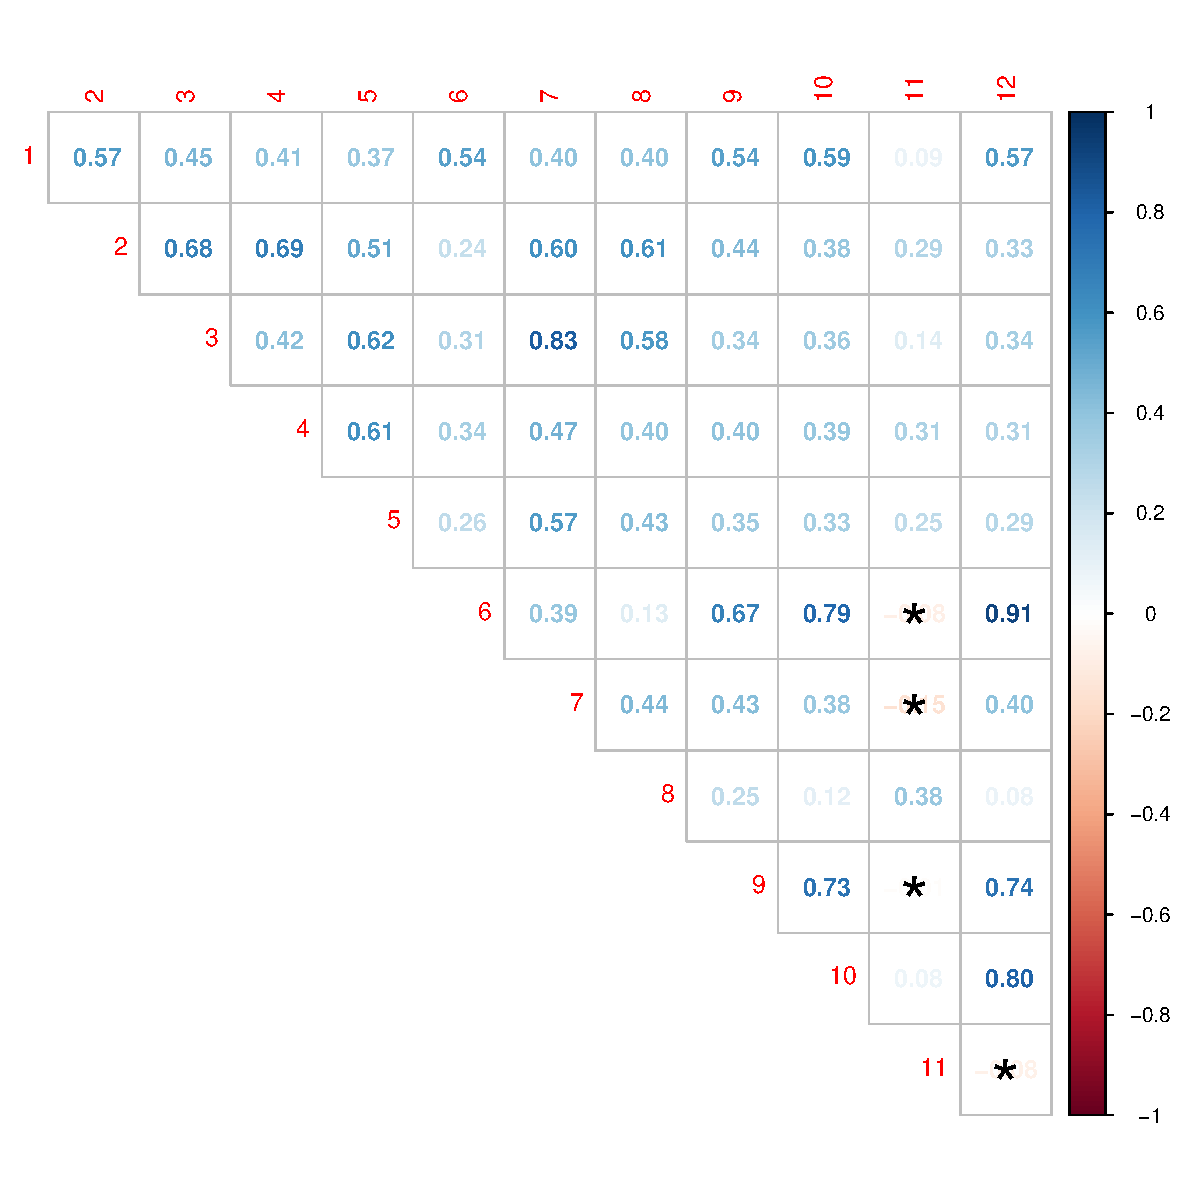
\includegraphics{analise_avaliacao_files/figure-latex/unnamed-chunk-2-1} \end{center}

\hypertarget{anuxe1lise-de-cluster}{%
\section{Análise de cluster}\label{anuxe1lise-de-cluster}}

\begin{center}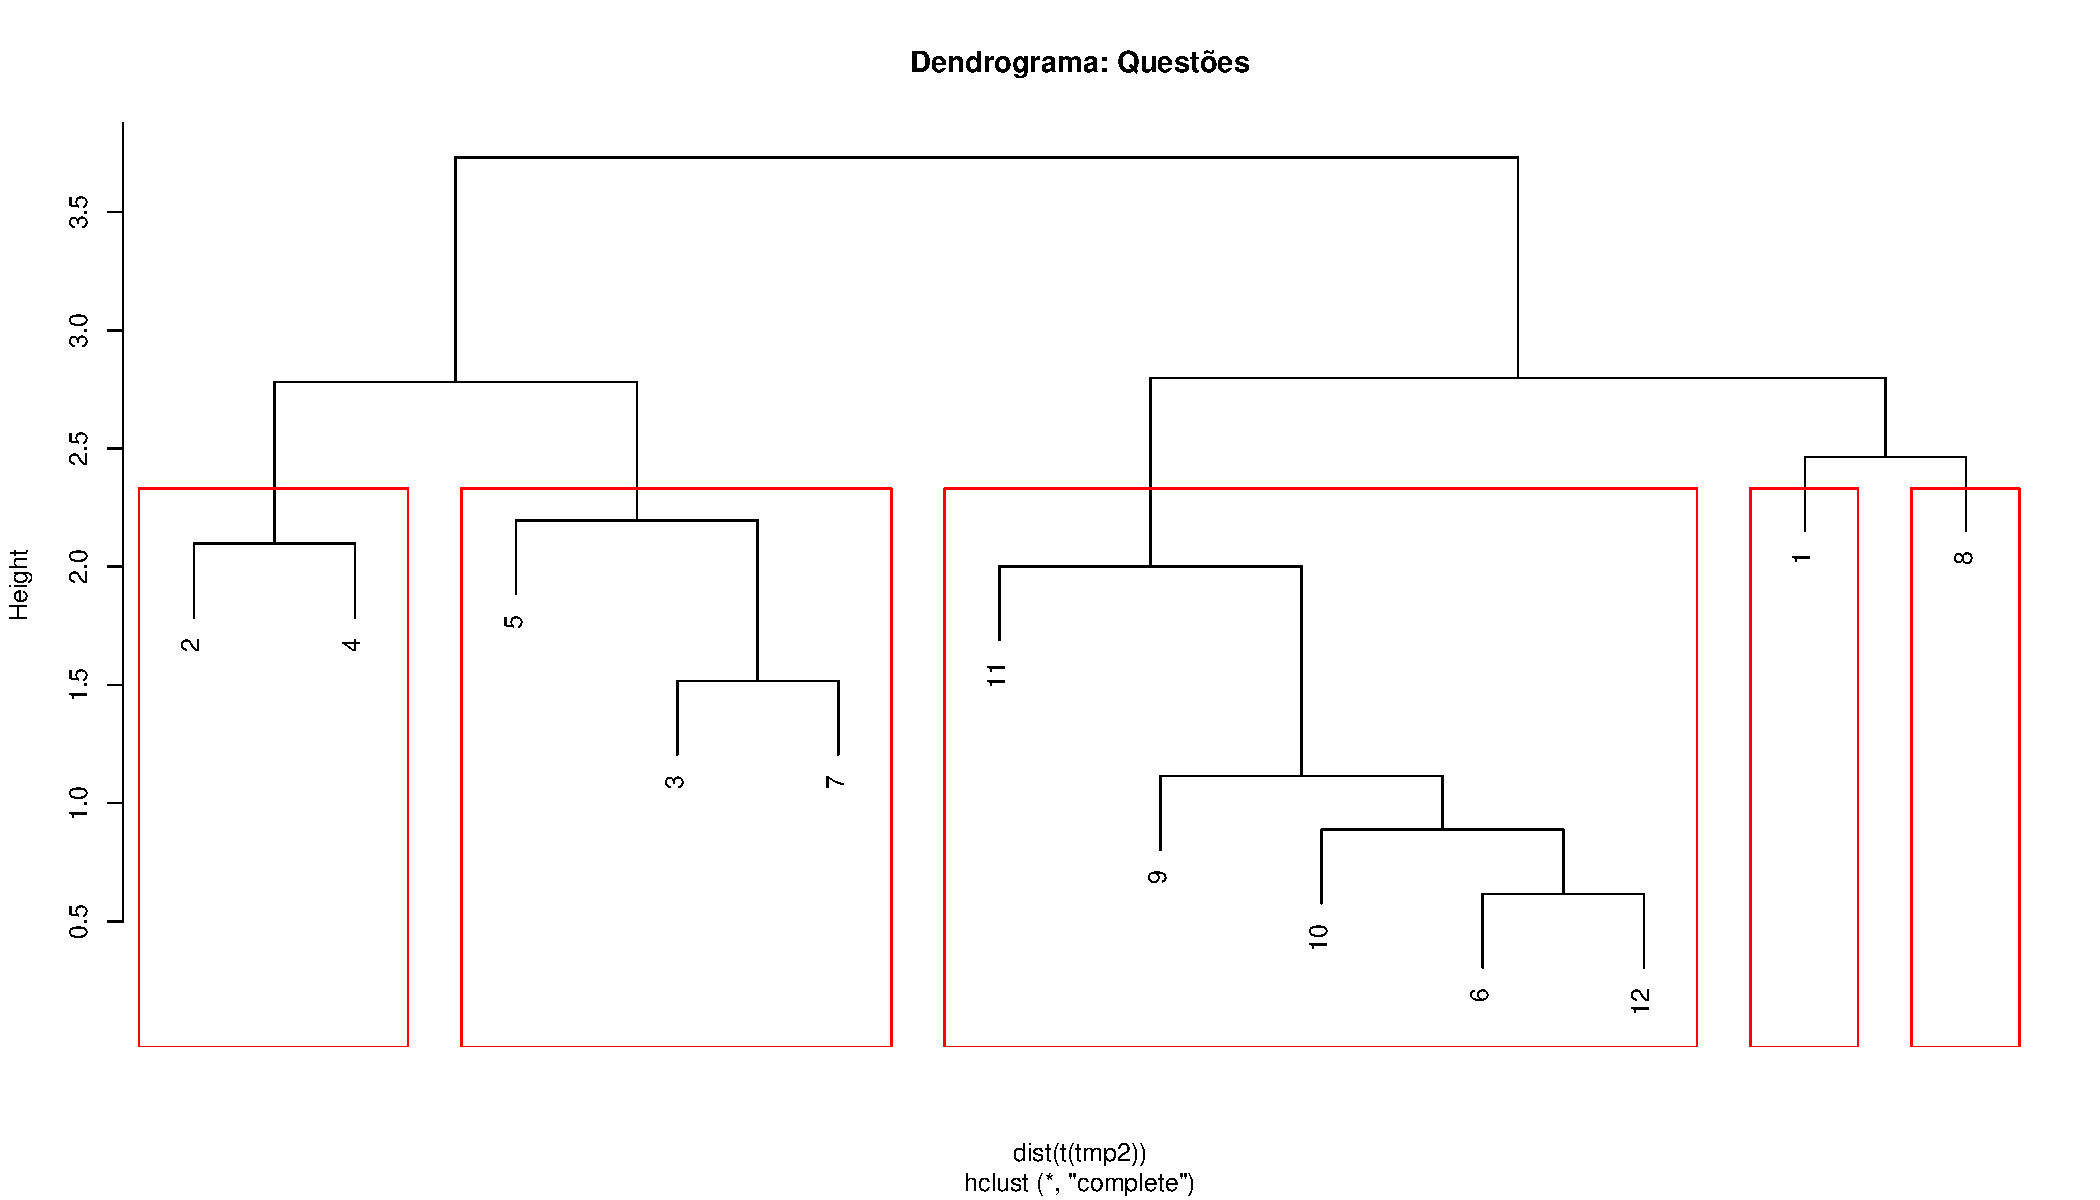
\includegraphics{analise_avaliacao_files/figure-latex/unnamed-chunk-3-1} \end{center}

\begin{center}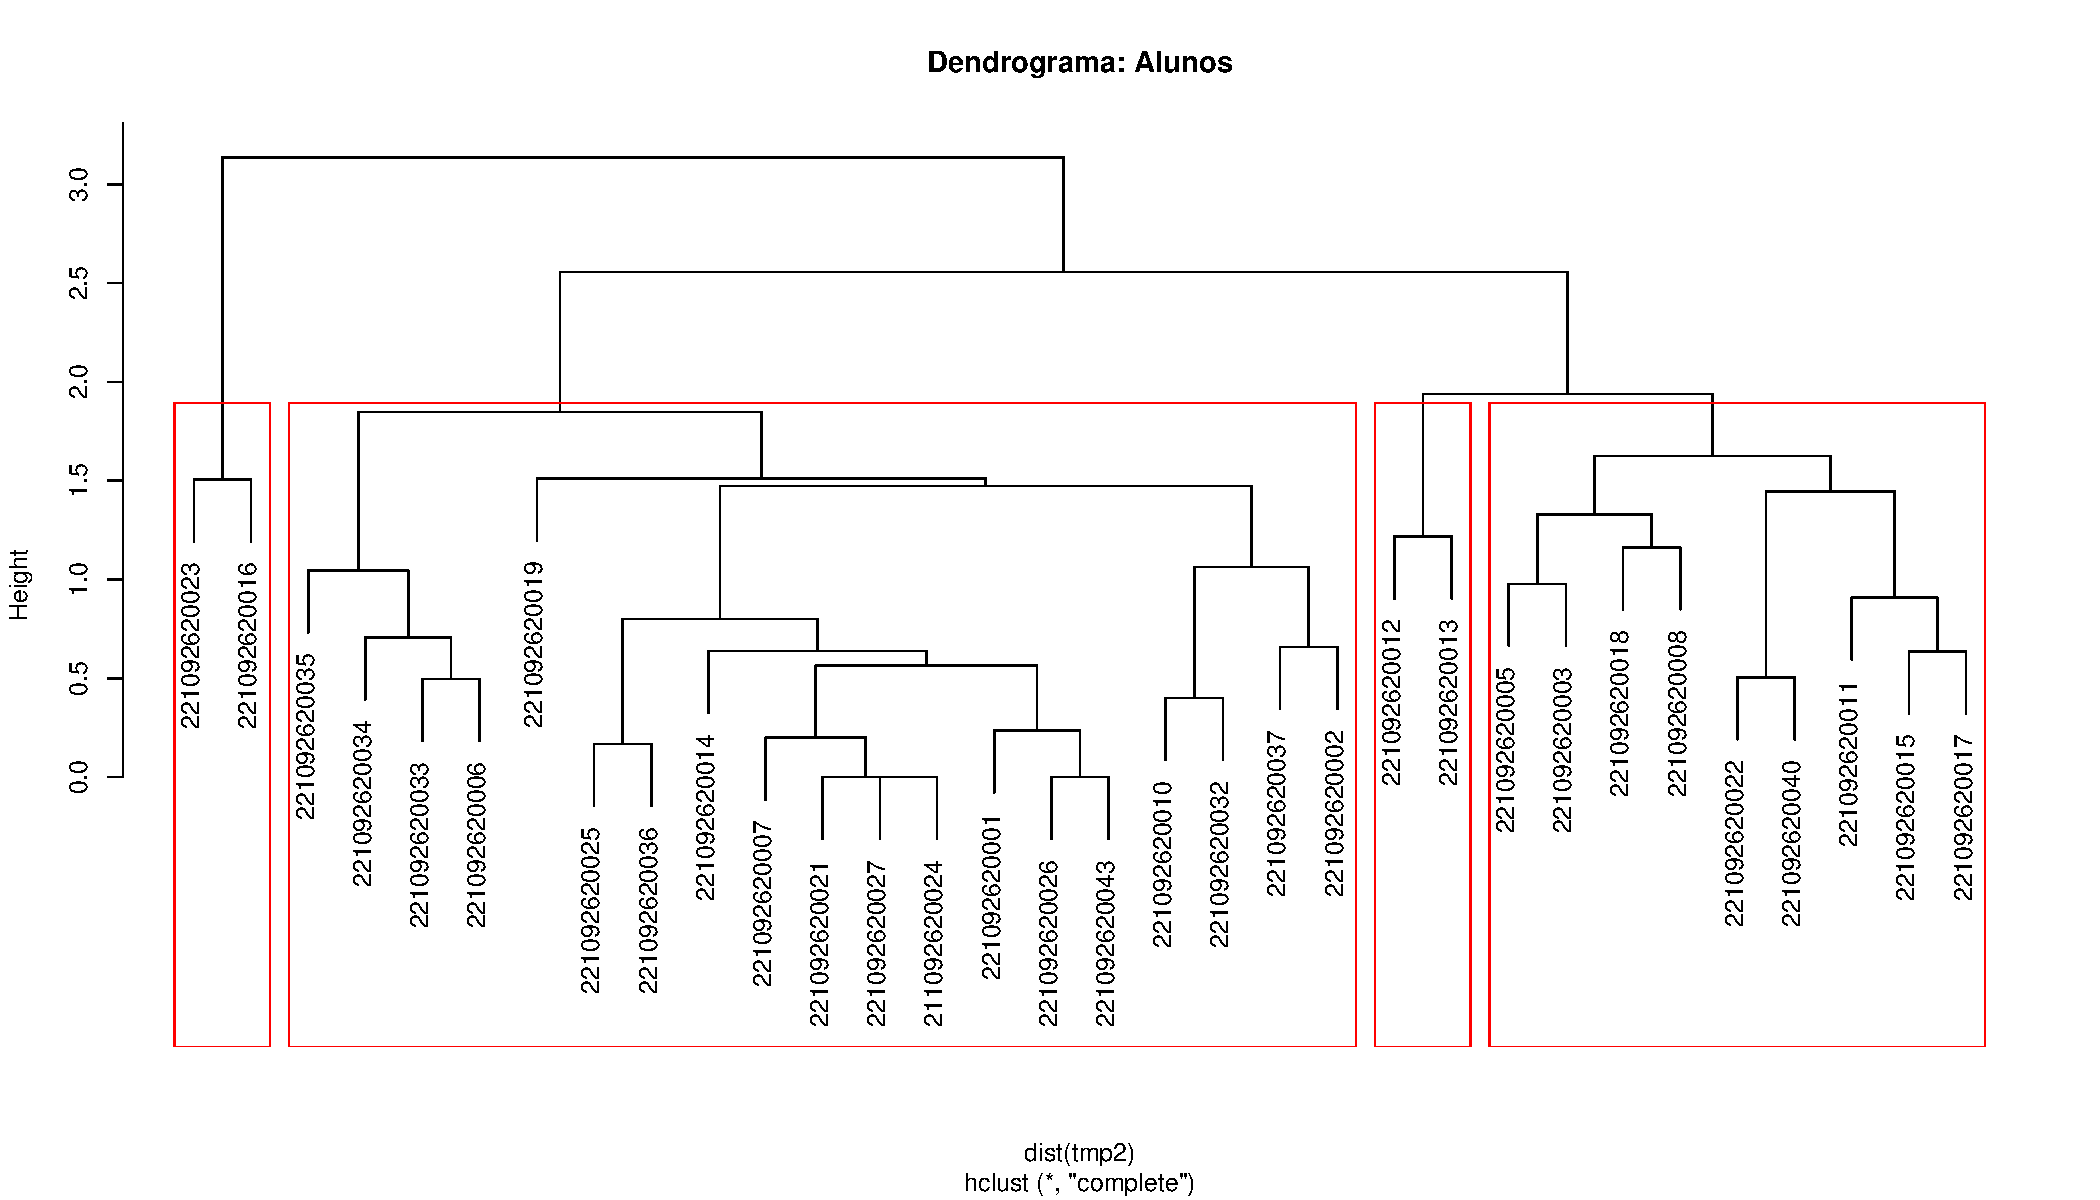
\includegraphics{analise_avaliacao_files/figure-latex/unnamed-chunk-3-2} \end{center}

\end{document}
